\section{Methods}

\subsection{Model}

In the MBD model, parameters $\lambda$ and $\mu$ correspond, respectively, 
to the common per-species speciation and extinction rates present 
also in the standard BD model. 
Additionally, MBD relies on two additional parameters. 
Parameter $\nu$ is the rate at which an environmental change is triggered.
When such event is triggered, each species present in the phylogeny at that 
moment has a probability $q$ to speciate at that time.
This kind of speciation is of a different nature respect to the one triggered 
by $\lambda$. In fact, whereas parameter $\lambda$ can be seen as describing 
a sympatric process, $\nu$ induces the rise of geographical barriers 
interrupting the gene flow and leading to an allopatric speciation.
Even though multiple speciations can co-occur, polytomies are not allowed 
in such process as each species can speciate only once at the time.
A likelihood expression for the process is provided in \cite{mbd}.

\subsection{Tree simulations}

We can easily simulate such processes in continuous time using the 
Doob-Gillespie algorithm. Simulations are performed using the 
function "mbd\_sim" from the \verb;mbd; package (\citep{mbd}).
We let parameters vary using all possible combinations of values
as shown in Table~\ref{tab:simulation_parameters}.
For each parameter setting, we simulate $1000$ independent trees.

We have picked the parameters in such a way that in the most speciose
setting, the simulated trees have usually less than 200 taxa.

\begin{table}[ht]
  \centering
  \begin{tabular}{ | c | l | }
    \hline
    \textbf{Parameter} &
    \textbf{Values} \\ 
    \hline
    $\lambda$ & (0.2) \\
    $\mu$ & (0, 0.15) \\
    $\nu$ & (1.0, 1.5, 2.0, 2.5) \\
    $q$ & (0.1, 0.15, 0.2) \\
    crown age & 10 \\
    \hline
  \end{tabular}
  \caption{
    Parameters used to simulate MBD trees. For each parameter setting $1000$ trees are simulated.
  }
  \label{tab:simulation_parameters}
\end{table}

\subsection{Pirouette}

Once the MBD dataset has been simulated we exploit the \verb;pirouette; 
package (\citep{pirouette}) to assess the error made by BEAST2, executing 
the inference using a BD tree prior.

We briefly summarize here how the \verb;pirouette; routine works.
From each MBD tree a DNA sequence alignment is simulated. 
For each sequence alignment we then perform a Bayesian inference 
analysis (using BEAST2) to recover a posterior distribution of trees. 
For each parameter setting, this process leads to an inference error 
distribution. To evaluate the extent of this error we also run 
a \verb;pirouette; "twin" pipeline, through which we mimic the original 
pipeline in every aspect but starting instead from "twin" trees.
From each MBD simulated tree we can produce its BD twin, inferring the most 
likely BD parameters (i.e. $\lambda$ and $\mu$) through maximum likelihood, 
and use them to simulate a standard BD tree (see \cite{pirouette} for more 
information), keeping the topology of the original tree.
We let the Bayesian analysis assume a BD prior in both cases, to investigate 
the extent of the error we make under this assumption. The twin pipeline 
serves as an estimation of the baseline error, as its error it is not due by 
the mismatch of the generative prior with the inference prior.

\iffalse
\subsection{Model selection}

We simulate alignments using the simplest nucleotide substitution model (JC69),
the simplest clock model (strict). It is thus imminent to assume these
models in our Bayesian inference. Nevertheless, the phylogeny the alignment
was based on, could have followed either an MBD or BD tree model, 
where we in both cases assume a BD tree model. This will have 
an unknown effect on our inference: it may theoretically be that an MBD model
generates (a tree that generates) an alignment in which a different site 
and/or clock model is favored. 

We investigate this by measuring if the generative model (with the simplest
nucleotide substitution and simplest clock model) is indeed selected 
to be the best fitting model. 
To be precise, we look at the model 
with the highest marginal likelihood 
(also called evidence \cite{mackay2003information}),
$f(D|M)$, which is the probability of the data D given model M.
In the context of this research, D consists of the DNA alignment,
and M is the combination of site, clock and tree models.

To estimate the marginal likelihood, 
we use an algorithm named nested sampling \cite{skilling2006nested}.
Nested sampling is attractive to use
in a phylogentic context, as it gives a good estimation,
requires little tuning \cite{maturana2018}.
Nested sampling is available as a BEAST2 package
and can be used by babette \cite{babette}.

The nested sampling algorithm stops its run 
when the marginal likelihood estimation error 
reaches below a certain tolerance.  
Similar to \cite{maturana2018},
we use a (relative) error tolerance $\epsilon$ of $10^{-13}$,
1 particle to explore the parameter space
and 100 active points. 
To achieve the latter, we use the MCMC chain length $L_c$ of 1M 
(as also used in the parameter estimates),
and a sub-chain length $L_{sc}$ of 10K.

The models we use in our model comparison are the four combinations
of two site models and two clock models. We use the JC69 site model, which
is the (generative and) simplest model and GTR, the site model with most
degrees of freedom. For the clock models, we use the strict clock model,
which is the (generative and) simplest clock model, and the RLN clock model.
\richel{Could also just be all site models and clock models = 8 models}

From these four marginal likelihood estimates, we calculate the weight of
the generative model and plot this in figure 2. We do this for both the 
alignments derived from the MBD tree and the BD twin tree. We expect that
the generative model has the heighest weight in both the MBD and BD alignments.
We expect this weight to be higher in the BD alignments.
\fi

\subsection{Quantifying the impact of the speciation model}
\richel{this is a proposal}

To quantify the impact of the speciation model, we propose to
use impact = complete error - baseline error / complete error.



\begin{figure}[!htbp]
  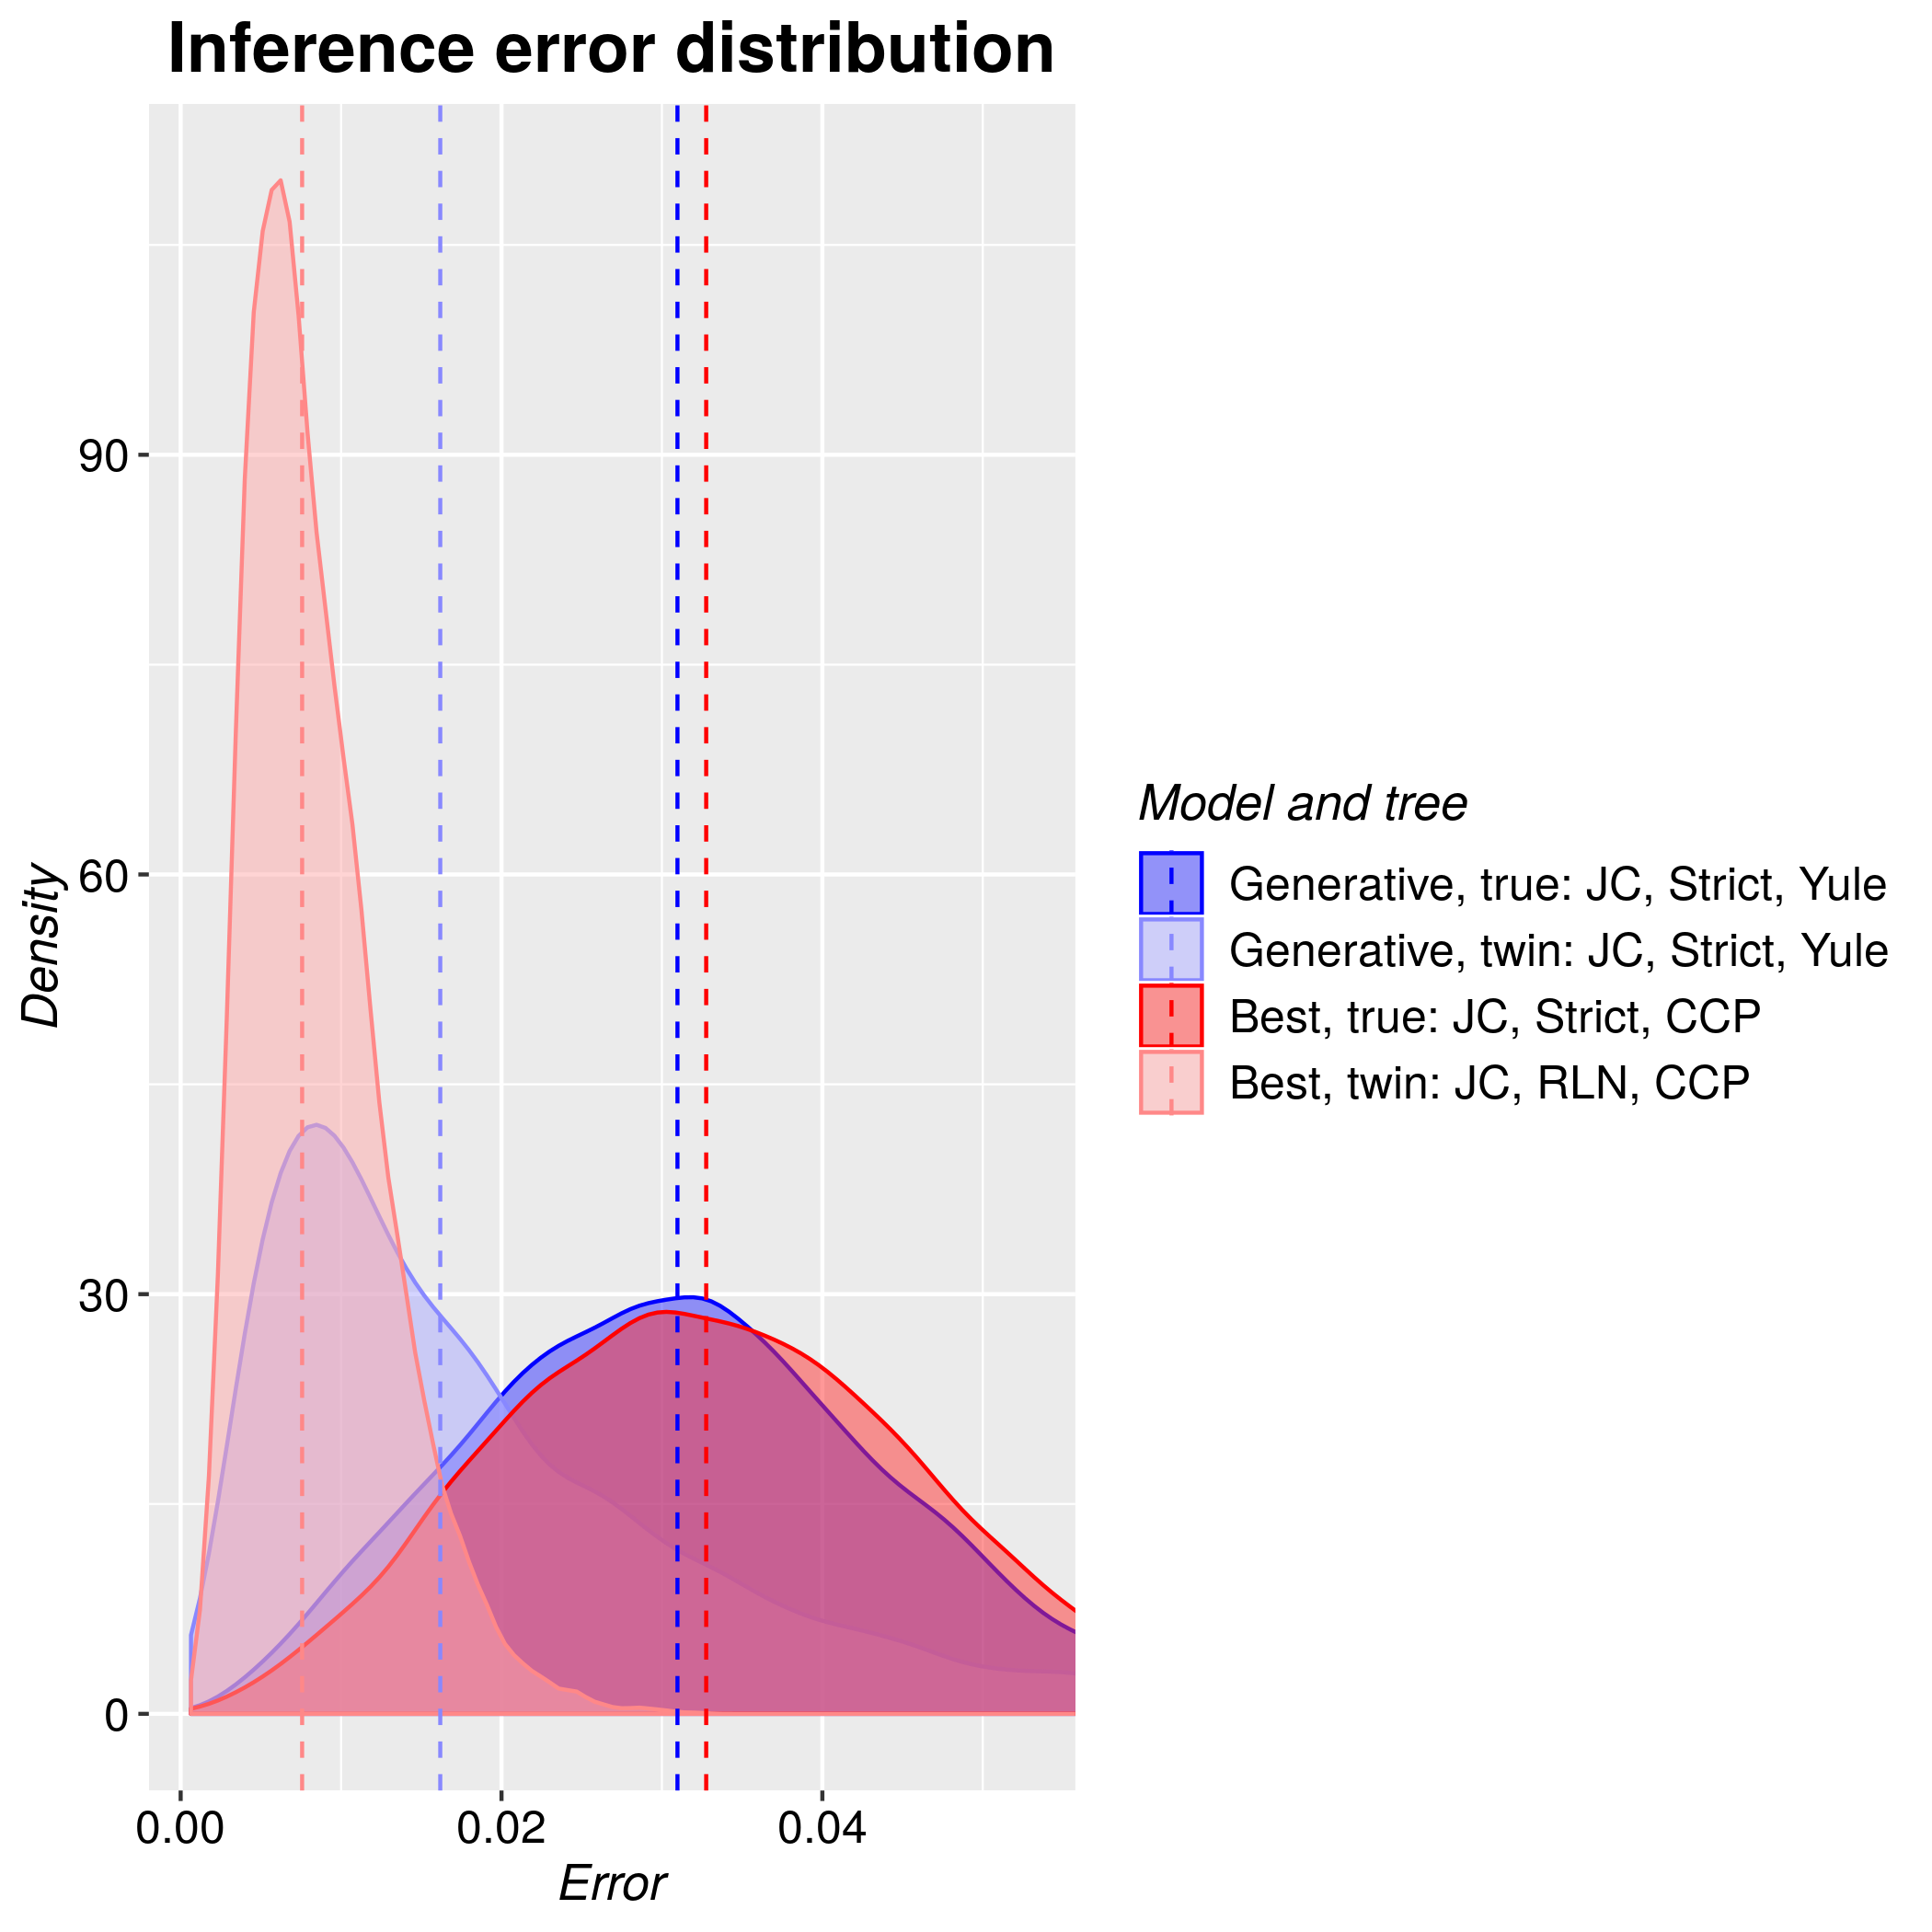
\includegraphics[width=\textwidth]{razzo-figures/pir_ex_3_errors.png}
  \caption{
    Uses Yule tree, impact of speciation model should be low
  }
  \label{fig:results}
\end{figure}

\begin{figure}[!htbp]
  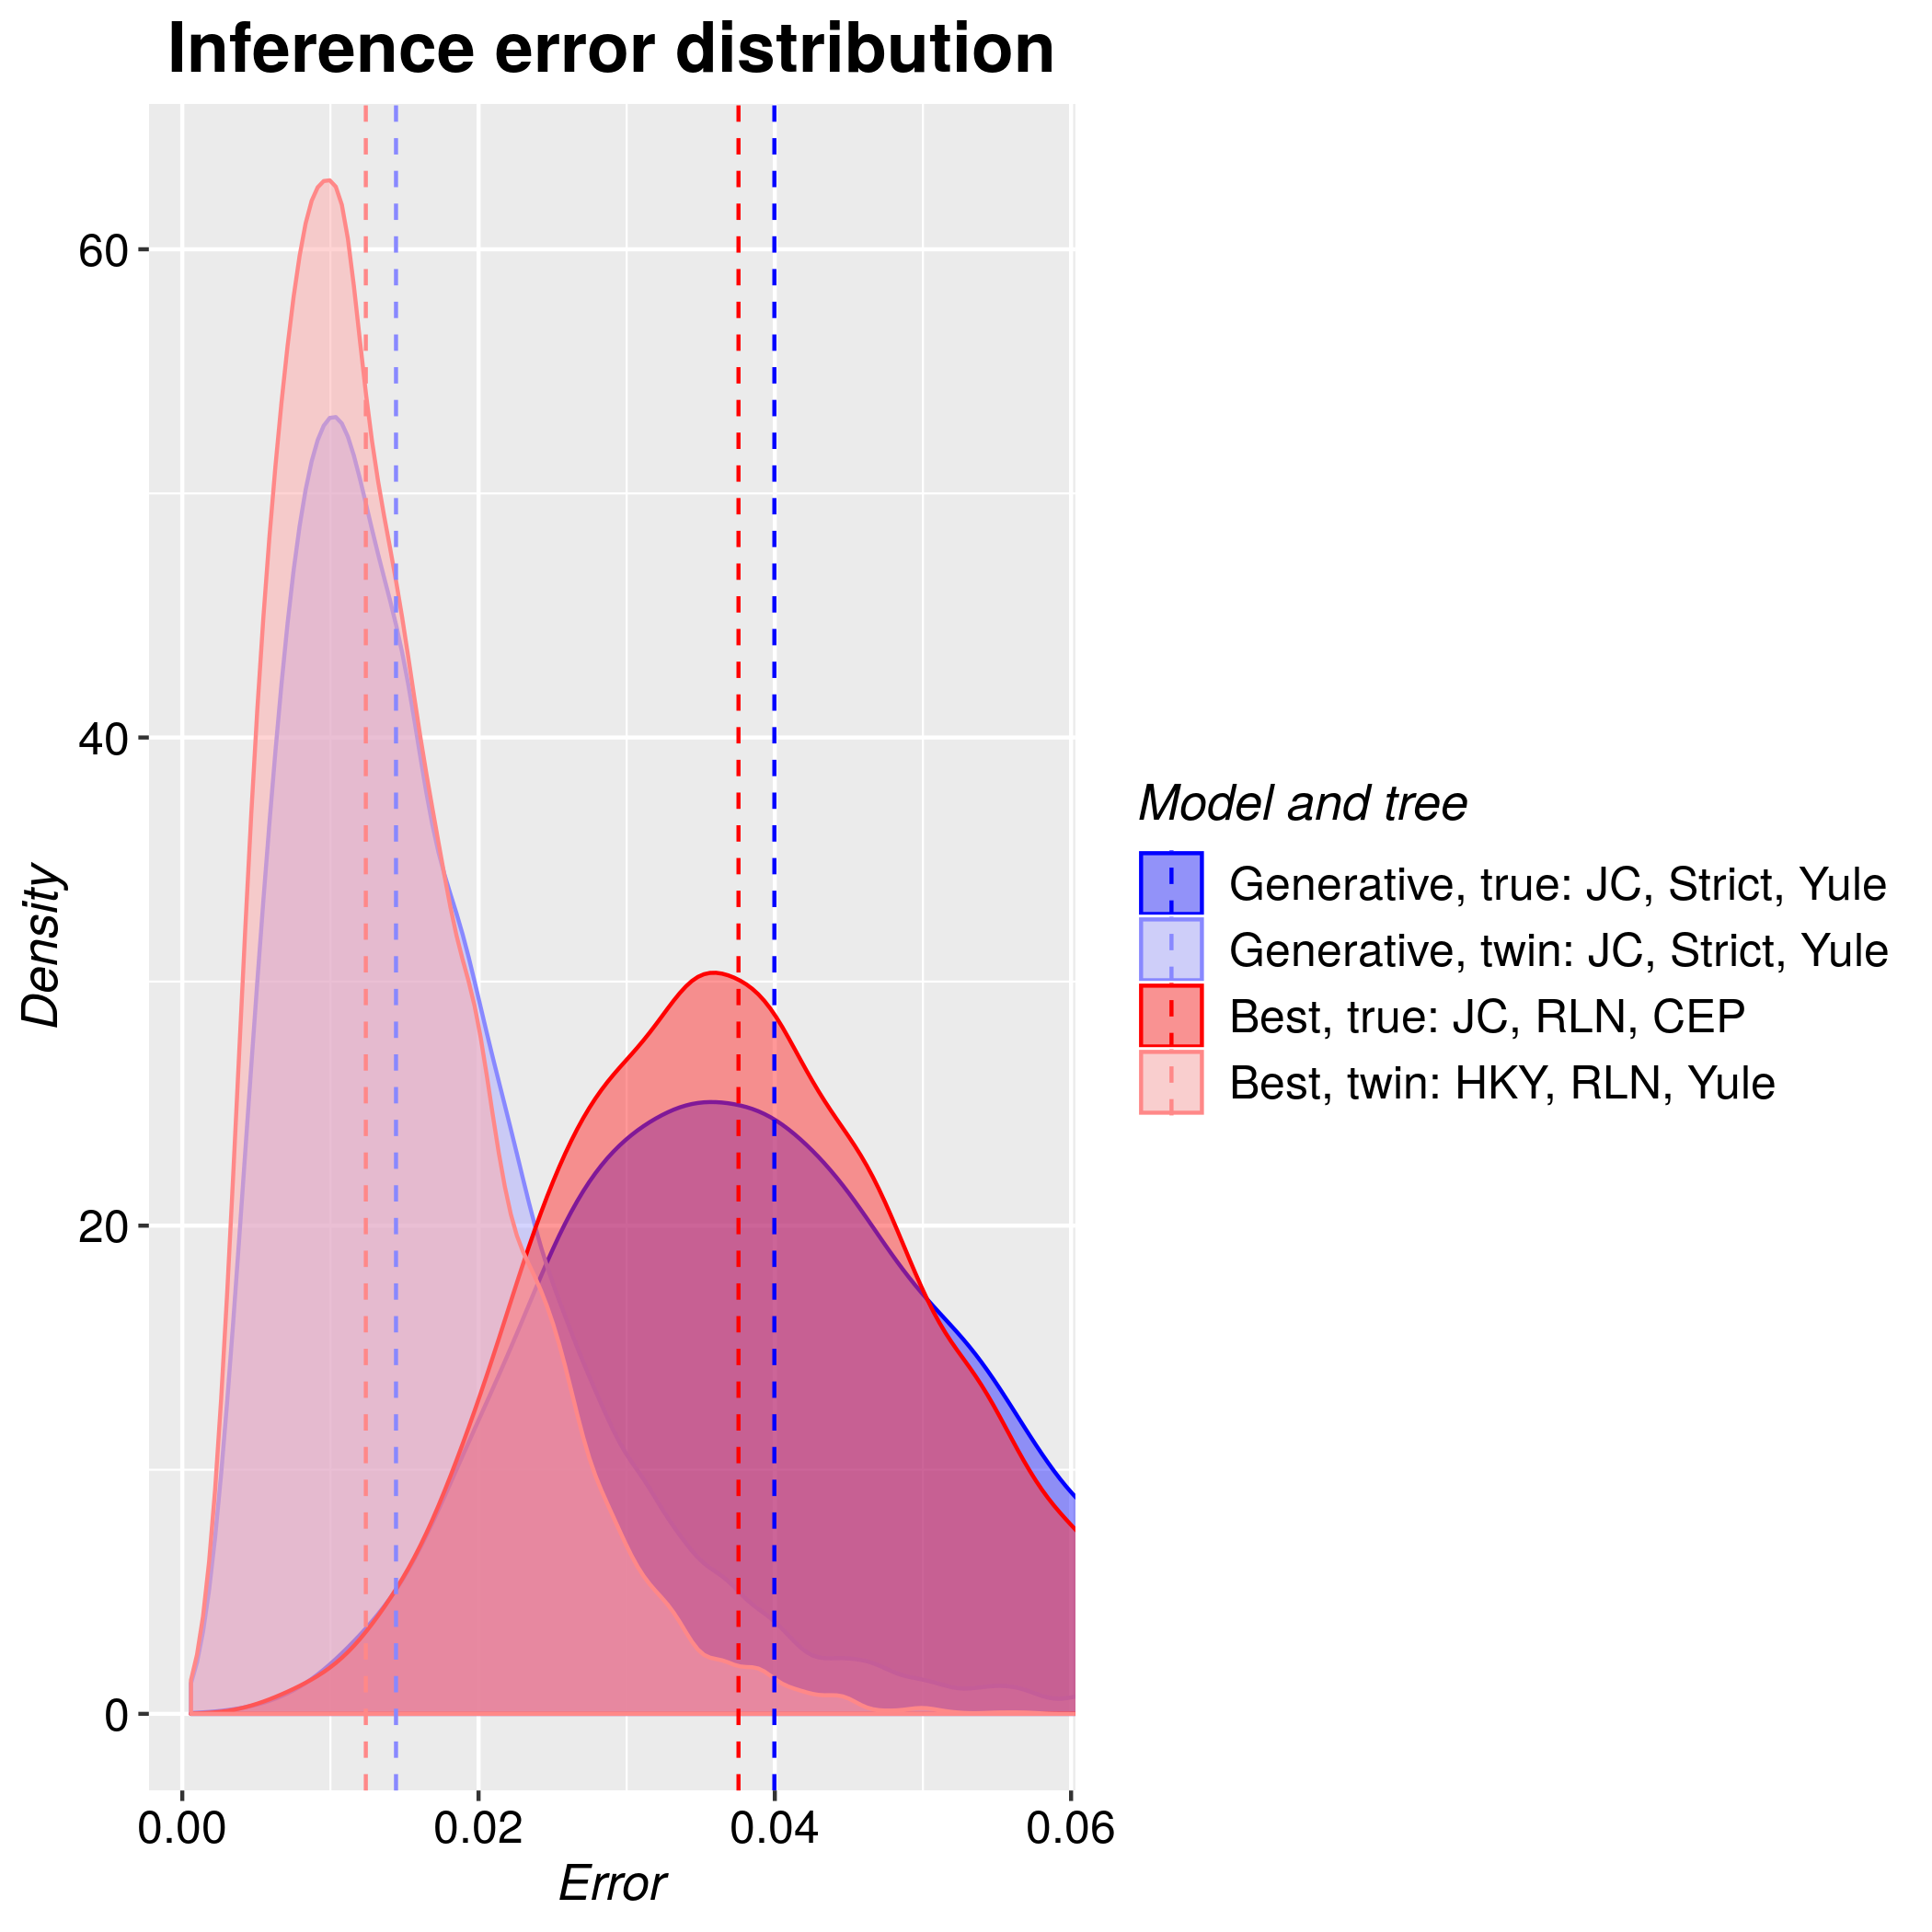
\includegraphics[width=\textwidth]{razzo-figures/pir_ex_6_errors.png}
  \caption{
    Uses non-standard tree, impact of speciation model should be high
  }
  \label{fig:results}
\end{figure}